\section{The LHCb detector}

The LHCb detector is a particle detector with the main focus on decays in which $b$ or $c$ quarks are involved.
Its goals are precision measurements on the CP-violation and on rare decays. 
To accomplish this, it has been build as a single arm forward-spectrometer covering angles to the beam pipe from $\qty{10}{\milli\radian}$ to $\qty{300}{\milli\radian}$ \cite{LHCb}. 
This design has been chosen because the majority of high energetic $b$-/$c$-hadron pairs, produced in $pp$~collisions, have velocities in roughly the same direction as one of the incident protons.
An overview of the detector is shown in \autoref{fig:lhcb_detector}.
The following paragraphs briefly describe the components of the LHCb detector based on the article \enquote{The LHCb Detector at the LHC}\cite{LHCb}.

\begin{figure}
    \centering
    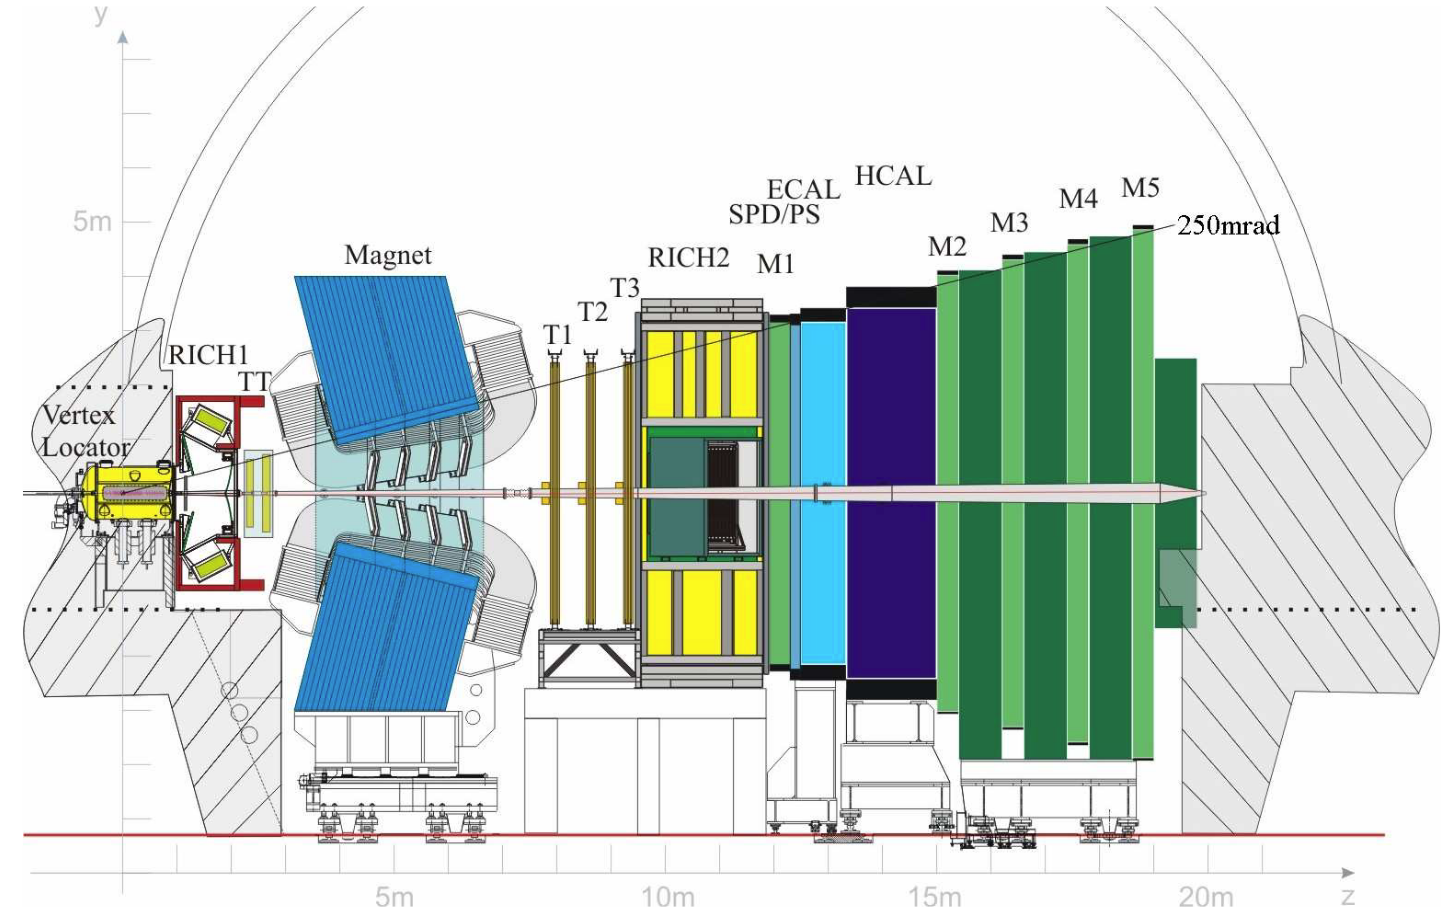
\includegraphics[width=\textwidth]{images/lhcb_detector.png}
    \caption{View of the LHCb detector \cite{LHCb}. }
    \label{fig:lhcb_detector}
\end{figure}

A particle produced at the primary vertex first traverses the Vertex Locator (VELO). 
There, the tracks of charged particles are measured using silicon semiconductor sensors at a resolution of about $\qty{4}{\micro\meter}$. 
This information then is primarily used to reconstruct the position of the primary and secondary vertices of the decay particles.

Beyond the VELO, the Tracking System then further measures the position over time of the same particles. 
This is done in the Tracker Turicensis (TT) before the magnet and in the Trackers T1, T2 and T3 behind the magnet.
The dipole magnet bends the particle tracks through the Lorentz force so that the particles' momentum can be inferred.
While the TT and the inner parts of the T1-T3 also use silicon semiconductor sensors, the outer parts of the T1-T3 use straw-tube modules which are gaseous ionization detectors. 

The Ring Imaging Cherenkov detectors (RICH1, RICH2) are used to measure the particle velocities.
By traversing optically dense materials, charged particles can induce the emission of Cherenkov radiation.
This radiation is then detected by photo multipliers. 
The opening angle of the circular emitted radiation is dependent on the velocity of the particle. 
The use of aerogel, $\symup{C}_4\symup{F}_{10}$ and $\symup{C}\symup{F}_4$ as radiators allows measuring particles with momenta between $\qty{1}{\GeV}$ and $\qty{100}{\GeV}$.
Comparing the momentum measured in the Tracking System with the velocity measured in the RICH detectors yields information about the particle identity based on its mass. 

The calorimeters (SPD/PS, ECAL, HCAL) stop most particles and measure their energy.
In dense materials particles induce particle showers with the size directly related to the energy deposited.
Each calorimeter is structured in alternating layers of absorbers and scintillators. 
The electronic calorimeter~(ECAL) absorbs electrons, positrons and photons using lead, and the hadronic calorimeter~(HCAL) absorbs any hadrons using iron.
The pad/preshower detector~(SPD/PS) is used to reject $\pi$~background detected in the ECAL.
The calorimeters are the only detectors at LHCb which can detect chargeless particles, and they are critical for particle identification.

The muon chambers (M1-M5) stop and track charged particles which pass through the calorimeters without absorption.
The only charged particles at this point in the detector are muons.
Iron layers are used to stop the muons and multi-wire proportional chambers  are used to detect them.

The only known particles that pass through the LHCb detector undetected are neutrinos.
They are indirectly measured through analysis of the missing transversal momentum and energy. 

A LHCb component not listed in \autoref{fig:lhcb_detector} is the Trigger System.
This system is needed to reduce the $\qty{40}{\MHz}$ beam crossing rate of the LHC to the $\qty{2}{\kHz}$ event detection rate of the LHCb. 
It consists of a hardware trigger (L0) and a software trigger (HLT).
The L0 collects information about the number of primary vertices from the pile-up system of the VELO.
It also attempts to reconstruct the highest $E_\text{T}$ in the calorimeters and the two highest $p_\text{T}$ in the muon chambers. 
This information is used to reject events until a detector read out rate of $\qty{1}{\MHz}$ is achieved.
The HLT then further triggers events asynchronously to this rate. 
For this, all detector outputs are evaluated for the involvement of $b$ hadrons in the events.
At the final rate of about $\qty{2}{\kHz}$, the event data is permanently written to hard drives and can be accessed on demand by all members of the LHCb collaboration.

